%! Author = Team Park
%! Date = \today

% Preamble
\documentclass{beamer}

\usetheme{Madrid} % This is a simple and clean theme, but you can change it to other themes like: Berlin, Warsaw, etc.

\title{CNN-Based Classifier for Speech Command Recognition}
\subtitle{A Deep Learning Approach to Audio Classification}
\author{Team Park: D. Hörtenhuber, O. König, W. Laube}
\institute{JKU \\ MLPC}
\date{\today}

\begin{document}

\begin{frame}
  \titlepage
\end{frame}

\begin{frame}{Introduction and Data Preprocessing}
  \begin{itemize}
    \item \textbf{CNN Overview:} CNNs are deep learning models effective in feature extraction from raw data, ideal for spectrograms.
    \item \textbf{Data Preprocessing:}
      \begin{itemize}
        \item \textit{Spectrogram Conversion}: Converting raw audio into spectrograms for input into the CNN.
        \item \textit{ICA for Noise Reduction}: Applying Independent Component Analysis to reduce background noise and improve signal quality.
      \end{itemize}
  \end{itemize}
\end{frame}

\begin{frame}{CNN Architecture and Training}
  \begin{itemize}
    \item \textbf{CNN Architecture:}
      \begin{itemize}
        \item \textit{Layers}: Convolutional layers, pooling layers, fully connected layers.
        \item \textit{Key Hyperparameters}: Filter sizes, number of layers, activation functions.
      \end{itemize}
    \item \textbf{Training Process:}
      \begin{itemize}
        \item \textit{Data Split}: Training, validation, and test set splits to ensure robust evaluation.
        \item \textit{Optimizer}: Adam optimizer with dropout regularization to prevent overfitting.
      \end{itemize}
  \end{itemize}
\end{frame}

\begin{frame}{Performance Evaluation}
  \begin{itemize}
    \item \textbf{Evaluation Metrics:} Accuracy, precision, recall, F1-score.
    \item \textbf{Results:}
      \begin{itemize}
        \item \textbf{Validation Set:}
          \begin{itemize}
            \item Accuracy: 92\%
            \item Precision: 92\%
            \item Recall: 91\%
            \item F1-score: 79\%
          \end{itemize}
        \item \textbf{Test Set:}
          \begin{itemize}
            \item Accuracy: X\%  % Replace with actual value
            \item Precision: Y\%  % Replace with actual value
            \item Recall: Z\%  % Replace with actual value
            \item F1-score: W\%  % Replace with actual value
          \end{itemize}
        \item \textbf{Comparison with Other Models:}
          \begin{itemize}
            \item Random Forest: Accuracy 89\%  % Replace with actual value
            \item Nearest Neighbour: Accuracy 45\%  % Replace with actual value
          \end{itemize}
      \end{itemize}
  \end{itemize}
\end{frame}

\begin{frame}{Confusion Matrix and Learning Curves}
  \begin{itemize}
    \item \textbf{Confusion Matrix:}
      \begin{figure}
        \centering
        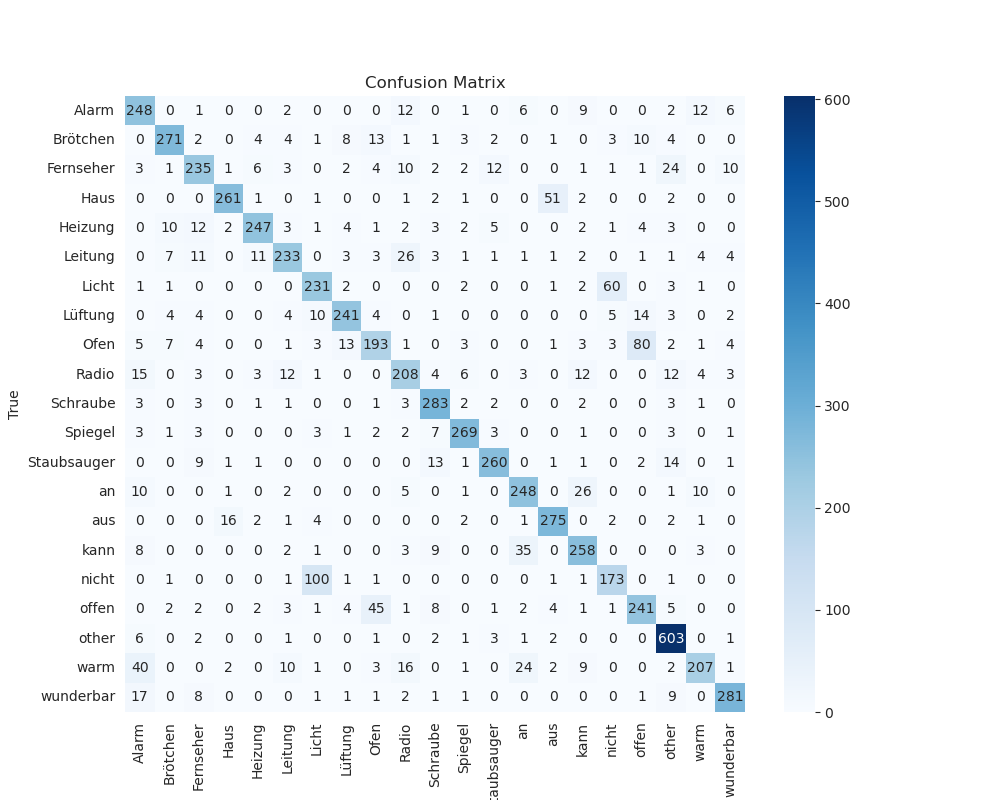
\includegraphics[width=0.8\textwidth]{confusion_matrix.png}
        \caption{Confusion Matrix for 1D CNN}
      \end{figure}
    \item \textbf{Learning Curves:}
      \begin{figure}
        \centering
        \includegraphics[width=0.8\textwidth]{learning_curves.png}
        \caption{Learning Curves for 1D CNN}
      \end{figure}
  \end{itemize}
\end{frame}

\begin{frame}{Analysis and Conclusion}
  \begin{itemize}
    \item \textbf{Qualitative Analysis:} Performance on realistic scenes, highlighting strengths like noise handling and any observed weaknesses.
    \item \textbf{Conclusion and Future Work:}
      \begin{itemize}
        \item \textit{Summary}: CNN achieved high accuracy and robustness.
        \item \textit{Future Improvements}: Enhancing the model architecture, experimenting with different preprocessing techniques.
      \end{itemize}
  \end{itemize}
\end{frame}

\end{document}
